\section{Marked observations and integral monodromy}\label{sec:inverse}

We specify two inverse problems. The first recovers
projective bundle transport on a known graph.
The second recovers an unknown incidence graph and
then the integral monodromy of the curve family.
Both use component averages of low eigensections,
in addition to eigenvalues. The integral conclusion
also uses the known first-order smoothing and the
orientation of the base loop. These observations
are substantially richer than an unordered spectrum.

\subsection{The component-trivial construction on other graphs}
We first record the geometric hypotheses needed
to apply the preceding arguments beyond the quartic.

\begin{proposition}\label{prop:fixed-graph-extension}
Let $\pi:\mathcal Y\to\Delta$ be a proper holomorphic
nodal curve family with smooth total surface,
connected smooth fibres, and a reduced central
fibre with smooth normalization components $Y_i$.
Suppose its finite dual graph is connected and
has no self-edges, every node has coordinates
$u_ev_e=t$, and the fibre metrics are induced
by a fixed smooth Kähler form on the total surface.
Use component-trivial flat bundles with constant
$\SU(r)$ incidence maps on the exterior/node cover.

Then the spectral, finite-flow, actual-flow and
entry results of Sections~\ref{sec:spectrum}--\ref{sec:entry}
hold with $m=|V|(r^2-1)$, component areas $A_i$,
and all weights equal to $2\pi/L$,
$L=\log(1/|t|)$. Constants may depend on the
fixed family and rank. If $b_1(\Gamma)\ge2$,
the metric and intrinsic-distance comparisons
of Theorem~\ref{thm:moduli-metric} hold on the
irreducible graph-gluing locus. That locus is
Lagrangian when all $Y_i$ are rational.
\end{proposition}
\begin{proof}
Choose disjoint node bidiscs and connected component
exteriors. Their only overlaps are the two disjoint
incidence collars at each node. Constant unitary
maps therefore give the flat bundle and parallel
determinant exactly as in
Proposition~\ref{prop:bundle}; properness makes
the cover contain the entire nearby fibres.
Van Kampen gives the quotient onto $\pi_1(\Gamma)$
by killing the patch groups.

The required analytic estimates use only this
cover and fixed component geometry. A node cut
at radius $a$ has area $O(a^2)$, logarithmic
length $L+2\log a$, and exact interpolation
energy $2\pi\|X_i-\Ad(U_{ij})X_j\|^2/(L+2\log a)$.
The zero-boundary estimate of
Lemma~\ref{lem:zero-boundary} is local in the
smooth ambient node chart. Fixed-component
Poincaré, trace and elliptic estimates give
\eqref{eq:lower-energy} and \eqref{eq:low-mass}
with the new finite number of vertices.
The same min--max and dimension argument
gives exactly $m$ weak modes and the gap.

The product matrix space is now $\cP_r^{|V|}$.
Its finite potential, convexity and coercivity
are unchanged sums over this graph. On each
fixed closed $Y_i$, the mean-zero Green functions
have precisely the logarithmic singularity and
integral estimates used in
Section~\ref{sec:actual-flow}. The construction
therefore gives the same integrated residual,
trace comparison and all-time estimate under
the normalized spectral lower bound.
The fixed-component phase theorem holds on any
of these compact curves. Its preparation
construction uses only finitely many such flows,
fixed-coordinate collars and the node area
bound, so the same open initial class defined
by the extension norm and the
diagonal preparation time apply.

Finally, the proof of
Theorem~\ref{thm:moduli-metric} uses the
patch-trivial representation, affine
primitives, fixed exterior trace inequalities
and the common annular length. These hypotheses
are all present. Its quotient dimension is
$(b_1(\Gamma)-1)(r^2-1)$.
The radial representatives remain isotropic;
if every component is rational, the smooth
genus is $b_1(\Gamma)$ and the dimension is
half that of the surface moduli space.
\end{proof}

\subsection{The measured operator}
For the quartic with independent node lengths,
let $\mathcal S_{\tau,U}$ be the first $m$
eigenspaces, counted with multiplicity and
including the exact kernel. More precisely,
this is the $m$-dimensional spectral subspace
below the uniform complementary threshold.
On a fixed exterior of component $i$ choose
a parallel unitary frame. Fix a small cutoff
$a_0$ and define the averaging map
\[
 (T_{\tau,U}s)_i
 =\frac{1}{\operatorname{Area}(\Omega_i(a_0/2,\tau))}
       \int_{\Omega_i(a_0/2,\tau)}s_i\,dA_\tau .
\]
Its target $\cV$ carries the area inner
product $M$. The observations are the first
$m$ eigenvalues and the columns of $T_{\tau,U}$
in an $L^2$-orthonormal eigenbasis, together
with the known component labels, areas,
local frames and normalized node parameters.
No identification of component frames
across a node is observed.

\begin{lemma}\label{lem:marked-operator}
The map $T=T_{\tau,U}$ is invertible for
small parameters, and
$\|T^*T-I\|\to0$ uniformly in $U$ and
all node-length ratios. Set
\[
 G=TT^*,\qquad J=T^*G^{-1/2},\qquad
 \widehat B_{\tau,U}
       =J^*(\Delta_{\tau,U}|_{\mathcal S_{\tau,U}})J .
\]
Adjoints on $\cV$ use $M$.
Then $J$ is an isometry and
\begin{equation}\label{eq:marked-operator}
 \|\widehat B_{\tau,U}-B_{\tau,U}\|_M=o(w_*),
 \qquad w_*=\max_e w_e=\frac{2\pi}{L_*}.
\end{equation}
All these matrices are determined by the
declared observations and are independent
of the chosen orthonormal eigenbasis.
For the common-neck families of
Proposition~\ref{prop:fixed-graph-extension}
the same assertion holds with
$w_*=2\pi/L$.
\end{lemma}
\begin{proof}
The energy of every unit vector in the
low space is at most $Cw_*$.
Let $b^{(a)}$ be the means at a smaller
fixed radius $a<a_0/2$ used in
Lemma~\ref{lem:low-mass}.
The two averaging regions have a common
fixed positive-area subset. Poincaré on
the larger truncated component gives
\[
 \|b^{(a)}(s)-Ts\|_M\le C_a\sqrt{w_*}\,\|s\|_{L^2}.
\]
The low-space mass estimate consequently
gives
$|\|Ts\|_M^2-\|s\|^2|
\le(Ca^2+o_a(1))\|s\|^2$.
Let the parameters tend to zero and then
$a\to0$. This proves the uniform
asymptotic isometry and invertibility.
The polar formula gives $J^*J=I$ and
$TJ=G^{1/2}$.

Apply \eqref{eq:lower-energy} at the
fixed radius $a_0$ to $Jv$.
Writing $H=G^{1/2}$ and
$\beta_\tau=(1+C_{a_0}\sqrt{w_*})^{-2}$,
we obtain the quadratic-form inequality
\[
 \widehat B_{\tau,U}
       \ge D_{\tau,U}:=\beta_\tau H B_{\tau,U}H .
\]
Since $\|B_{\tau,U}\|_M\le Cw_*$,
we have $\|D_{\tau,U}-B_{\tau,U}\|_M=o(w_*)$.
Relative spectral comparison gives
$\tr\widehat B_{\tau,U}-\tr B_{\tau,U}=o(w_*)$.
The difference $\widehat B-D$ is
positive semidefinite in fixed dimension,
and hence
\[
 0\le\|\widehat B-D\|_M
       \le\tr(\widehat B-D)=o(w_*).
\]
This proves \eqref{eq:marked-operator}.
Eigenvalues alone would not identify the
operator in these component markings;
the polar construction uses the observed
averages. Changing an orthonormal basis
of a repeated eigenspace leaves the
construction unchanged.
\end{proof}

Let $\mathsf A=\operatorname{diag}(A_iI_d)$
in orthonormal component matrix coordinates,
$d=r^2-1$. The ordinary symmetric matrix
$\mathsf Q_{\tau,U}=\mathsf A B_{\tau,U}$
represents the finite energy. Its observed
version is $\widehat{\mathsf Q}=\mathsf A\widehat B$.
For a simple graph its off-diagonal blocks
satisfy
\begin{equation}\label{eq:offdiag-inverse}
 -(\mathsf Q_{\tau,U})_{ij}
       =w_e\Ad(U_{ij})\quad(e=ij).
\end{equation}

\begin{theorem}\label{thm:projective-inverse}
For the known simple graph and component
matrix-algebra markings induced by the
unitary frames, the observations above
recover projective edge transport
consistently whenever $w_e/w_*$ has a
fixed positive lower bound.
If
$\|\widehat{\mathsf Q}-\mathsf Q\|_{\op}
\le\delta w_*$, the recovered adjoint
edge map has error at most
$C\delta w_*/w_e$ for sufficiently small
such ratios of error to weight.
In particular all projective edge and
cycle transports are recovered uniformly
on the common-neck slice, even through
reducibility. The cycle representation
is recovered up to root conjugation.
\end{theorem}
\begin{proof}
Divide the observed block in
\eqref{eq:offdiag-inverse} by $w_e$.
Project it, in Frobenius norm, onto the
compact embedded group $\Ad(\SU(r))$.
Nearest-point projection is unique and
smooth in a fixed tubular neighborhood
of this compact submanifold of the
real matrix space. Norm equivalence in
fixed dimension and
\eqref{eq:marked-operator} give the
stated error. The marking specifies
the matrix algebra and therefore this
particular adjoint subgroup.
Since $\Ad(\SU(r))\simeq\operatorname{PSU}(r)$,
these are projective transports.
An error in a cycle product is bounded
by the sum of the edge errors, because
all projected and exact factors are
orthogonal. Tree transport then identifies
the root representation. Component frame
changes act by vertex gauge, giving
the stated conjugation ambiguity.
\end{proof}

This is asymptotic recovery with an error
bound, not exact reconstruction from one
finite-parameter observation.
For an edge with $w_e/w_*\to0$,
\eqref{eq:marked-operator} alone is
insufficient after division by $w_e$.
Relative eigenvalue control does not
remove this observation-conditioning issue.
The areas are fixed known positive
numbers; uncertainty or unbounded
variation in them is not included.

Central twists are exactly invisible.
Multiplying edge maps by elements of
the center of $\SU(r)$ leaves the
adjoint connection and every marked
observation unchanged on each fibre.
For fixed projective edge maps the
choices of lifts, modulo central vertex
changes, form an $H^1(\Gamma;Z(\SU(r)))$
torsor before further stabilizer
identifications. Thus an $\SU(r)$ lift
cannot be inferred from these data.

\subsection{Compact families with unknown incidence}
Take six labelled copies of $\PP^1$,
each with three branch points at
$0,1,\infty$. Pair their eighteen branch
points according to a connected simple
trivalent graph on the six vertices.
The observer is given the components
and unpaired branch points, but not
the pairing. We use the finite class
of these pairings, including the
triangular prism and $K_{3,3}$.

\begin{proposition}\label{prop:common-local-metrics}
Every such pairing has a proper projective
holomorphic smoothing with smooth total
surface, first-order node equations
$uv=t$, and connected genus-four smooth
fibres. One can choose smooth ambient
Kähler forms so that every normalization
component has the same prescribed
area-one Fubini--Study metric and every
smaller node bidisc has the same metric
germ. Component-trivial flat $\SU(r)$
bundles with arbitrary unitary edge
maps exist on these entire families.
\end{proposition}
\begin{proof}
Every central rational component has
three distinct nodes, so the curve is
stable and its arithmetic genus is
$9-6+1=4$. The proper flat analytic
plumbing of
\cite[Section~8.3 of the preprint version]{hubbard-koch}
uses independent node parameters;
restrict to their diagonal $t_e=t$.
Concretely, glue product exteriors to
disjoint node bidiscs by
$(u,t)\mapsto(u,t/u)$ and its reverse.
For $|t|<a^2$ the incidence collars at
a node are disjoint. Smaller closed
exterior cores and node bidiscs cover
the fibres over each closed smaller
parameter disc, which also verifies
properness. The total space is smooth
because $uv-t$ has nonzero $t$
derivative at a node, and is a product
away from the nodes. Connectedness
of the graph gives connected smooth
fibres.

The relative dualizing line bundle is
invertible and has degree one on each
central component. Its cube is very
ample and has vanishing first
cohomology on every fibre by
\cite[Theorem~1.2]{deligne-mumford}.
Riemann--Roch gives fifteen sections.
The analytic base-change theorem
\cite[Section~7, Satz~5]{grauert}
applies to this proper flat family
over a reduced disc and the line
bundle, which is flat over the base,
with constant section
dimension. Its direct image is
locally free of rank fifteen.
After shrinking and trivializing it,
evaluation embeds the family in
$\PP^{14}\times\Delta$.
Fibrewise very ampleness separates
the nodal tangent directions; the
base coordinate supplies the remaining
direction. This proves relative
projectivity of the analytic plumbing.

An embedding alone would not give
identical local metrics for different
pairings. To arrange that, use the
fixed $\mathcal O(1)$ and Fubini--Study
metric on each component. Choose
unitary Möbius coordinates at the
three branch points: $z$ at zero,
$(z-1)/(z+1)$ at one, and $1/z$ at
infinity. In suitable holomorphic
frames their squared metric is
$(1+|u|^2)^{-1}$.
Pull these line bundles to the
product exteriors and use a trivial
line on each node bidisc. Identify
the chosen branch frames with its
frame on the incidence collars.
There are no triple overlaps, so
these identifications define a
holomorphic line bundle on the
entire restricted family.

On a node give its frame squared norm
\[
 |e|^2=\bigl((1+|u|^2)(1+|v|^2)\bigr)^{-1}.
\]
On the $u$ overlap its ratio to the
component metric is $(1+|t/u|^2)^{-1}$.
Interpolate the logarithm of this
ratio on fixed disjoint collars.
It and all tangential derivatives
restrict to zero on the central
branch. The resulting smooth Hermitian
metric therefore has Chern form
$\Omega$ restricting to the prescribed
Fubini--Study form on every component,
and equal to
$\omega_{\mathrm{FS}}(u)+\omega_{\mathrm{FS}}(v)$
on each smaller node bidisc.

This form is positive near every node
and vertically positive on the compact
remainder of the central fibre.
In fixed submersion charts on that
remainder its vertical coefficient
is bounded below and its other
coefficients are bounded. The Schur
complement shows that
$\Omega+C\pi^*\omega_\Delta$ is positive
for a sufficiently large $C$.
The added term is nonnegative near
the nodes and vanishes on fibres.
Properness allows one smaller base
disc on which positivity holds
everywhere. Take the largest $C$
over the finite set of pairings.
The smaller-node germs and the
central component metrics are
then identical in their declared
coordinates.

Finally the same exterior/node cover
with constant special-unitary
incidence transitions gives the flat
bundles, parallel metric and determinant.
This construction verifies all the
hypotheses of
Proposition~\ref{prop:fixed-graph-extension}
on these families.
\end{proof}

On either graph one can take tree
maps equal to $I$, two free-cycle
maps equal to $(I+i\sigma_x)/\sqrt2$
and $(I+i\sigma_y)/\sqrt2$, and the
other two equal to $I$. They give
irreducible rank-two representations.
Thus these same compact families
carry stable bundles with genuinely
noncommuting gluing and the actual
HYM dynamics of the preceding
proposition.

\subsection{Incidence and the integral invariant}
For this inverse problem the data are
the six labelled unpaired components
with their local metrics and area
normalization, the rank, the normalized
parameter $t$, the fact that each
node is smoothed to first order,
and the positive orientation of the
base loop. Choose local parallel
orthonormal adjoint frames on fixed
component exteriors. Observe the
first $m=6d$ eigenvalues and their
orthonormal eigensection averages
there. The incidence matrix, global
vanishing cycles, cycle lattice and
monodromy are not part of the data.
Arbitrary orthonormal adjoint frames
suffice for this topology problem;
the stronger matrix-algebra marking
is needed only to recover projective
bundle transport.

\begin{theorem}\label{thm:monodromy-inverse}
For the finite family class of
Proposition~\ref{prop:common-local-metrics},
the declared observations recover
the labelled incidence graph exactly
for all sufficiently small $|t|$,
uniformly in all unitary transports.
They thereby determine the integral
symplectic conjugacy class of the
positive monodromy
$\mathcal T:H_1(C_t,\mathbb Z)\to H_1(C_t,\mathbb Z)$.
In particular they determine
$\operatorname{Tor}\operatorname{coker}(\mathcal T-I)$.
For the triangular prism and $K_{3,3}$
these groups are, respectively,
\[
 \mathbb Z/5\mathbb Z\oplus\mathbb Z/15\mathbb Z,
 \qquad
 (\mathbb Z/3\mathbb Z)^2\oplus\mathbb Z/9\mathbb Z .
\]
\end{theorem}
\begin{proof}
The component areas are one.
Let $W_t$ have the measured average
columns and put $S_t=W_tW_t^*$.
Lemma~\ref{lem:marked-operator} gives
invertibility for small $t$ and
the consistent estimator
\begin{equation}\label{eq:unknown-incidence-estimator}
 \widehat Q_t
 =\frac1{2\pi}S_t^{-1/2}W_t
     \operatorname{diag}(L\lambda_0,\ldots,L\lambda_{m-1})
                          W_t^*S_t^{-1/2}.
\end{equation}
This formula contains no edge list.
For each underlying graph it satisfies
$\|\widehat Q_t-Q_{\Gamma,U}\|_{\op}\to0$,
where
\[
 \langle Q_{\Gamma,U}X,X\rangle
       =\sum_{ij\in E}\|X_i-\Ad(U_{ij})X_j\|^2.
\]
The maximum of the finitely many
family-dependent errors still tends
to zero uniformly in $U$.

Simplicity of the graph gives
$-(Q_{\Gamma,U})_{ij}=\Ad(U_{ij})$
on an edge and zero otherwise.
The Frobenius norms are $\sqrt d$
and zero. Define
\[
 ij\in\widehat E_t
 \quad\Longleftrightarrow\quad
 \|-(\widehat Q_t)_{ij}\|_{\mathrm F}
                                      >\tfrac12\sqrt d .
\]
An operator error less than $1/2$
gives a block Frobenius error less
than $\sqrt d/2$, proving exact
adjacency recovery. Independent
orthonormal frame changes preserve
these block norms. If the constructed
operator error is less than $1/4$,
any further operator perturbation
of norm less than $1/4$ preserves
the conclusion. This is an error
margin for the constructed operator;
raw measurement-noise propagation
through \eqref{eq:unknown-incidence-estimator}
is a separate question.

The recovered object is the labelled adjacency
graph. This does not determine which of the
three individually marked branch points is
attached to each neighbor. The integral
monodromy conjugacy class below depends only
on the graph and the prescribed smoothing
orders, so this remaining ambiguity does not
affect the stated inverse conclusion.

Orient the recovered edges and form
the integral incidence map
$B:\mathbb Z^E\to\mathbb Z^V$,
$B(e)=v_{\mathrm{head}}-v_{\mathrm{tail}}$.
Write
\[
 F=\ker B,\qquad C=\operatorname{im}B^T,\qquad
 F^*=\operatorname{Hom}(F,\mathbb Z)
              \simeq\mathbb Z^E/C.
\]
A spanning tree supplies an integral
fundamental-cycle basis and proves
the required saturation. The cycle
lattice $F$ and its dual $F^*$ are
not identified isometrically.

For rational normalization components
the integral degeneration sequence is
\begin{equation}\label{eq:integral-degeneration}
 0\longrightarrow F^*\simeq V_{\mathrm{van}}
 \longrightarrow H_1(C_t,\mathbb Z)
 \longrightarrow F\longrightarrow0 .
\end{equation}
Here $V_{\mathrm{van}}$ is generated
by the oriented vanishing loops
$\delta_e$, whose relations are
$\sum_eB_{ve}\delta_e=0$.
These are the normalization and
nearby-cycle descriptions in
\cite[Proposition~7.3.3 and Remark~7.4.2]{achinger-ogus}.
They can also be seen by cutting
the surface into the rational
component pieces and annuli:
the boundary relations at each
piece are the incidence relations,
and the remaining crossing cycles
are the graph cycles.
The quotient in
\eqref{eq:integral-degeneration}
is free, so $V_{\mathrm{van}}$ is
primitive. Its disjoint generators
make it isotropic; its rank four
is half the rank of $H_1(C_t,\mathbb Z)$.

Use the intersection convention
$\langle a_i,b_j\rangle=\delta_{ij}$
and positive local monodromy
\[
 \mathcal T(x)=x-\sum_e\langle x,\delta_e\rangle\delta_e .
\]
The coefficient of every node is
one because $uv=t$.
The integral Picard--Lefschetz
factorization
\cite[Theorem~7.4.1, Corollary~7.4.3
and Proposition~7.4.4]{achinger-ogus}
says that $N=\mathcal T-I$ kills
$V_{\mathrm{van}}$ and induces
\[
 q:F\longrightarrow F^*,\qquad
 q(c)(d)=\sum_e c_ed_e .
\]
Choose a fundamental-cycle matrix
$Z$ with integral basis columns
and set $G_\Gamma=Z^TZ$.
Choose the dual basis $a$ of
$V_{\mathrm{van}}$ and lifts $b$
of the cycle basis. Primitivity
permits integral symplectic lifts:
the skew intersection matrix of
initial lifts is removed by adding
integer combinations of the $a_i$.
In this symplectic basis,
\begin{equation}\label{eq:monodromy-matrix}
 \mathcal T=\begin{pmatrix}I&G_\Gamma\\0&I\end{pmatrix},
 \qquad N=\begin{pmatrix}0&G_\Gamma\\0&0\end{pmatrix}.
\end{equation}
The sign agrees with the chosen
positive loop and intersection
convention.

Changing the cycle basis by
$P\in\operatorname{GL}(4,\mathbb Z)$
replaces $G_\Gamma$ by $P^TG_\Gamma P$
and conjugates \eqref{eq:monodromy-matrix}
symplectically. Changing the lifts
does not alter the induced block.
Thus the graph determines the
claimed integral symplectic
conjugacy class, rather than a
matrix in an unprovided homology
marking. Reversing the base loop
would reverse the sign; that
orientation was declared as input.

The positive form $G_\Gamma$ need
not be unimodular. In particular
the image of $N$ need not be
primitive, although its saturation
$V_{\mathrm{van}}$ is. We have
\[
 \operatorname{Tor}\operatorname{coker}N
       \simeq F^*/q(F)
       \simeq\operatorname{coker}G_\Gamma.
\]
This is the graph critical group.
Its order is the spanning-tree
number; the cycle-lattice,
dual-lattice and critical-group
identifications are classical
\cite[Propositions~1, 3 and 7,
and Lemma~2]{bacher-harpe-nagnibeda}.
The explicit calculation below
gives the asserted groups.
\end{proof}

\subsection{Two identical local models}
Number the vertices $0,\ldots,5$.
The prism has triangles $012,345$
and matching edges $03,14,25$;
$K_{3,3}$ has every edge between
$\{0,1,2\}$ and $\{3,4,5\}$.
Orient every edge from its smaller
to its larger vertex and use
lexicographic edge order.
Choose the prism tree
$01,02,03,14,25$ and the bipartite
tree $03,04,05,13,23$.
For each remaining edge, use the
oriented chord followed by the
returning tree path. These four
cycles are an integral basis:
their chord submatrix is $I_4$,
and subtracting their chord
coefficients from any integral
cycle leaves a cycle on a tree,
which is zero.
Their Gram matrices are
\begin{equation}\label{eq:two-cycle-forms}
 G_{\mathrm{pr}}=
 \begin{pmatrix}
 3&-1&1&2\\-1&4&1&-2\\1&1&4&2\\2&-2&2&5
 \end{pmatrix},
 \qquad
 G_{\mathrm{bi}}=
 \begin{pmatrix}
 4&2&2&1\\2&4&1&2\\2&1&4&2\\1&2&2&4
 \end{pmatrix}.
\end{equation}
Exact integer arithmetic gives
\[
 \begin{array}{c|c|c|c}
 \text{graph}&
 \text{gcds of minors of orders }1,2,3,4&
 \text{Smith diagonal}&\det G_\Gamma\\ \hline
 \text{prism}&1,1,5,75&1,1,5,15&75\\
 K_{3,3}&1,3,9,81&1,3,3,9&81
 \end{array}
\]
Successive ratios of the minor gcds
give the Smith diagonal. The exact
calculation also verifies $BZ=0$,
the identity chord submatrix,
$N^2=0$, and preservation of the
standard symplectic form by
\eqref{eq:monodromy-matrix}.
All matrices and integer checks
are reproduced by the accompanying
computation.

\begin{figure}[t]
 \centering
 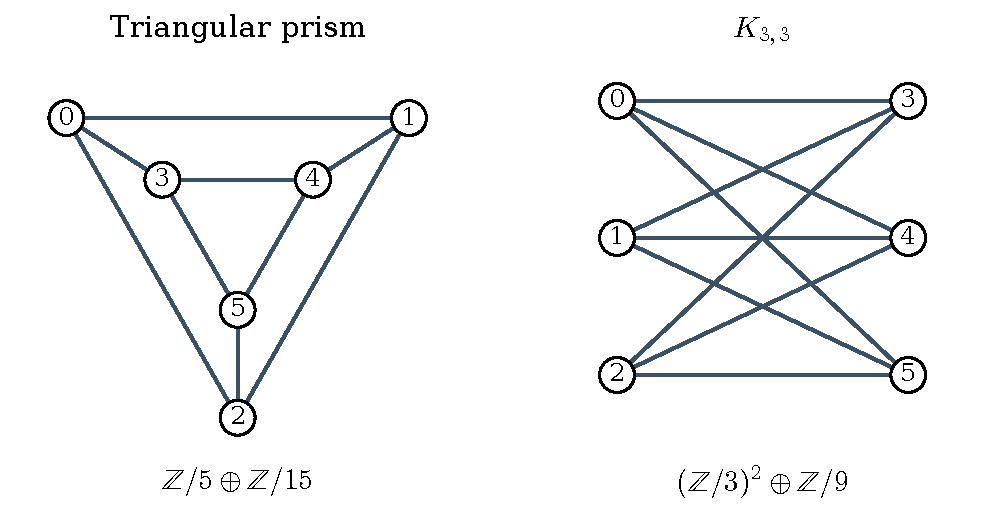
\includegraphics[width=\textwidth]{figures/output/monodromy-graphs.pdf}
 \caption{Two attachment graphs for the same six
 triply pointed rational components. The local
 component metrics and first-order node metric
 germs can be identical. The integral monodromy
 torsion groups have different orders, $75$ and $81$.
 The diagram depicts the exact attachment data;
 it is not a numerical spectral experiment.}
 \label{fig:monodromy-graphs}
\end{figure}

Both smooth fibres have genus four,
and their rational nilpotent
monodromy ranks are four.
Their smooth surfaces therefore
have the same diffeomorphism type.
What differs is an integral
invariant of the degeneration.
The local geometric inputs alone
do not determine it; the marked
global low-mode data determine
the missing adjacency and hence
the integral form.

This conclusion uses the full
Gram form for the conjugacy class;
the Smith diagonal records only
its cokernel group. Parallel
edges are excluded because sums
of their transported off-diagonal
blocks can cancel. Unknown
smoothing orders would change
the monodromy pairing to
$Z^T\operatorname{diag}(n_e)Z$
and require additional observations.
Neither the minimality of the
present observation package nor
recovery from unmarked eigenvalues
is asserted.
